\section{Gesamtübersicht}
\begin{figure}[H]
\centering
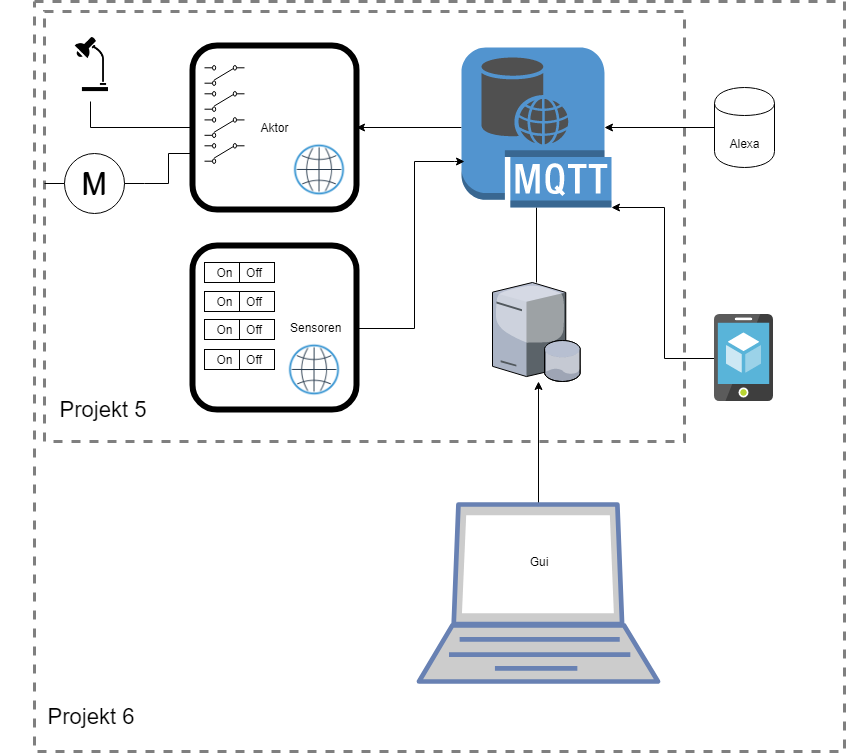
\includegraphics[width=\linewidth]{P5mqttAutomation.png}
\caption{Gesamtübersicht Projekt 5 und Projekt 6}
\label{pic: Gesamtübersicht}
\end{figure}
 In der Abbildung \ref{pic: Gesamtübersicht} sind im inneren Quadrat die Komponenten, für welche im Projekt 5 die Evaluationen ausgeführt werden. Dabei ist ein Aktor- wie auch ein Sensor-Print, die Kommunikation mit dem MQTT-Protokoll sowie der Inhouse Server für die Datenerfassung und Systemkonfigurationen enthalten. Im Projekt 6 werden die geplanten Komponenten ausgeführt und erweitert. Im Bereich welcher erweitert werden soll, ist eine Bedieneroberfläche (GUI) wie auch eine Steuerung mittels Smartphone und als Wunschziel Sprachsteuerung inbegriffen.